\begin{tcolorbox}[colback=yellow!10!white,colframe=red!50!black,fonttitle=\scshape,
  titlerule=0pt,
  title={\refstepcounter{exa}example~\theexa: Title of Example},
  title style={fill=yellow!10!white},
  coltitle=white, %red!50!black
  drop shadow]
  Hi, i am a yellow example
  \begin{center}
    \centering
    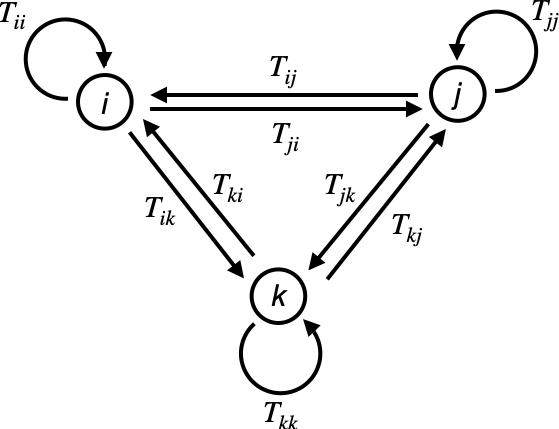
\includegraphics[width=0.99\textwidth]{figures/graph.png}
    \label{example:dice_entropy}
  \end{center}
\end{tcolorbox}
In example \ref{example:dice_entropy}

\begin{thesisbox}{The important concept}
\blindtext
\end{thesisbox}
\blindtext